\documentclass[a4paper,12pt,twoside]{article}



\title{Assignment 1b}

\author{Tung X. Nguyen}
\date{\today}

\setcounter{tocdepth}{3}


\usepackage{tikz,pgfplots}

\pgfplotsset{compat=1.10}
\usepgfplotslibrary{fillbetween}
\usepackage{apacite}
\usepackage{bm}
\usepackage{url}
\usepackage{amsmath}
\usepackage{indentfirst}
\usepackage{amssymb}
\usepackage[showframe=false]{geometry}
\usepackage{booktabs}
\usepackage{amsmath}
\usepackage{tabularx}
\usepackage{systeme}

\usepackage{graphicx}
\graphicspath{ {./img/} }

\usepackage[english]{babel}
\usepackage[utf8]{inputenc}
\usepackage{fancyhdr}
\setlength{\headheight}{15.2pt} 
 
\pagestyle{fancy}
\fancyhf{}
\fancyhead[LE,RO]{Tung X. Nguyen}
\fancyhead[RE,LO]{MAT9004: Assignment 1}
\fancyfoot[LE,RO]{\thepage}
\fancyfoot[CE,CO]{\leftmark}

\renewcommand{\headrulewidth}{2pt}
\renewcommand{\footrulewidth}{1pt}
\numberwithin{equation}{section}

\begin{document}
\maketitle
\thispagestyle{empty}

\tableofcontents
\listoffigures
\thispagestyle{empty}
\newpage

\oddsidemargin = 22pt
\evensidemargin = 22pt
\marginparsep = 10pt
\marginparwidth = 35pt


\section{Introduction}
\subsection*{1}
Basketball easily is one of the most favored kinds of sports ever been invented. The game is the most dominant in the United States, where the National Basketball Association, arguably the most competitive basketball league of the world, headquaters. Each regular season usually starts in October and finish in April. Then come the play-off, lasting from April to June and finally, the finals. The draft also happens in June, when young promising talents from over the world waiting for their name to be called.

In most types of sports, physicality is an important indicator of players for their potential to success. This is especially true for basketball, which is a very physical game. Even though basketball IQ and tatics play a vital role, it is the muscle that delivers the hardwork. NBA basketballs are, in general, not only huge but also exceptionally fit. This was not always the case. In the past century, basketball players were mostly tall, sometimes skinny men. As time goes by, we see more players with more body mass. This undeniable trend is a proof showing that physique in NBA is gaining more importance.

Inspired by this observation and by my interest in the game, I decided to pick "The importance of physique in NBA" as the topic for this report. In this report, I attemp to answer several key questions:
\begin{itemize}
\item What is the most common physique type in the NBA (2019-2020) by position, by height, by weight, wing size ...?
\item How physique can affect the draft number of a player? For instance: do bigger players get more chance of being picked in the first round?
\item How physique and Player Efficiency Rating correlated?
\item Is there any differences in the physique of non-US players to US players?
\end{itemize}



\section{Data Wrangling}
The data used for my projects are all scraped from online basketball websites mentioned in the subsection \textbf{Data sources}. I used Python with the help of libraries including Selenium, BeautifulSoup, pandas and csv to automatically surf the websites, scan for data, and finally write them down to dataframe that can be stored in text files and reused in the future.
\subsection{Data sources}
\subsubsection{NBA players regular season stats from Official NBA Statistics and Advanced Analytics}Link: \textit{stats.nba.com/players/bio/} 

This website contain the information about players' full name, their age, their draft, height and weight. There is also the information about their draft (including draft year, draft round, draft number) and key perfomance measurement and the team they are playing for, and these information usually changes season after season. 

\subsubsection{NBA Draft Combine Anthro}
Link \textit{stats.nba.com/draft/combine-anthro/}

This is a more detail table showing players' physicality index such as body fat percentage, wingspan, hands' length and width, height with shoes on and off. Not all players in the NBA show up in the Draft Combine Anthro. This data only applies to  young talents who are going to be drafted for the same year or the year after. This data is used to complement the bio dataset above. It is important to accept that the wingspan, hands' length and width, and standing reach are less likely to change over seasons, but the body fat percentage is.

\subsubsection{Player Efficiency Rating (PER)} 
Link \textit{insider.espn.com/nba/hollinger/statistics}.

This is a scale developed by John Hollinger, former Vice President of Basketball Operations for the Memphis Grizzlies (an NBA team). This all-in-one formula attempts to calculate a player's contribution per playing minute, taking in consideration key performance items such as field goals, assists, steals, blocks, rebounds, free-throw, three-pointers \cite{wiper}. PER is not the perfect scale to measure a player defensively (as good defensive players are not necessarily excellent blockers or stealers), but it is still one of the most popular tools available to do evaluate players. Figure 1 is a reference table for PER, provided by Hollinger himself.

\begin{figure}[h!]
\caption{PER reference guide}
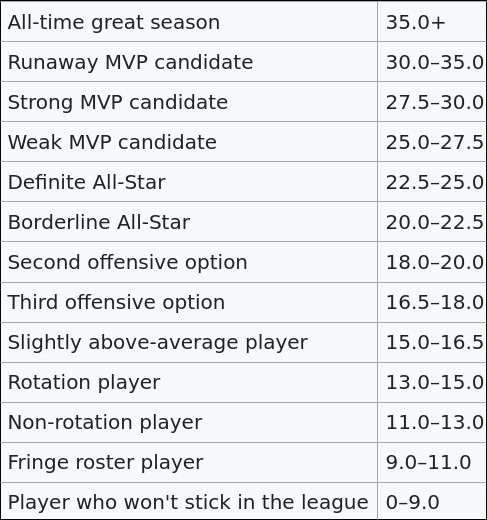
\includegraphics[scale=0.5]{hop.jpg}
\centering
\end{figure}

The PER dataset I used for this assignment is for regular seasons only. Available data includes: the number of games played, minutes per game, true shooting percentage, assist ratio, turnover ratio, usage rate, offensive/defensive rebound rate, PER, value aded, and estimated wins added. Explanation and formula for each of these columns can be found in the end of the data table on the website.


\subsection{Data Cleaning and Transformation}
After the data is saved to csv files, I proceed to transform them into the format I wanted. 

For the NBA players regular season data, I retained only the columns that contain data about physique and draft. Next, I perform union on datasets across seasons from 2000-2001 to 2019-2020 to finally get the data of total 1965 players playing in the NBA from 2000 to 2020. I then remove 57 entries that contains null in physique information. The \textbf{Height} column is originally in feet-inch format, so I used regex to extract tokens and transform this column in to a new column named \textbf{Height\_cm}. \textbf{Weight} is in pound unit.  The result is a dataframe like in Figure 2. The dataframe is sorted according to the \textbf{Draft Year} and \textbf{Draft Round} columns. It can be seen that there are many players who were undrafted, but I decided to keep all these entries (there are 562 undrafted players).

\begin{figure}[h]
\caption{NBA players from 2000 to 2020}
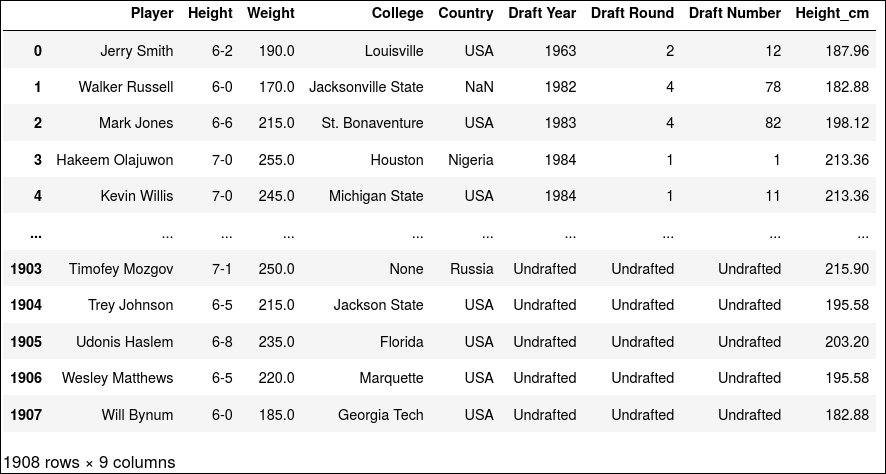
\includegraphics[scale=0.4]{nba_ap.jpg}
\centering
\end{figure}
For the NBA Draft Combine Anthro data, I also perform union to merge across seasons. It is worth noticing that the NBA Draft Combine Anthro started out with only Standing reach, Weight, and  Wingpsan. Body fat were then introduced in the season 2003-2004. Finally, in the season 2010-2011, Hand length and Hand width were added to the measurement. For this dataset, I only keep data about wingspan, hand length and width, standing reach and body fat percentage. I also convert the wingspan and standing reach from feet-inch to centimeters like I did for the regular season dataset. The last five entries in the resulting dataframe is shown in Figure 3.
\begin{figure}[!]
\caption{NBA Draft Combine Anthro from 2000 to 2020}
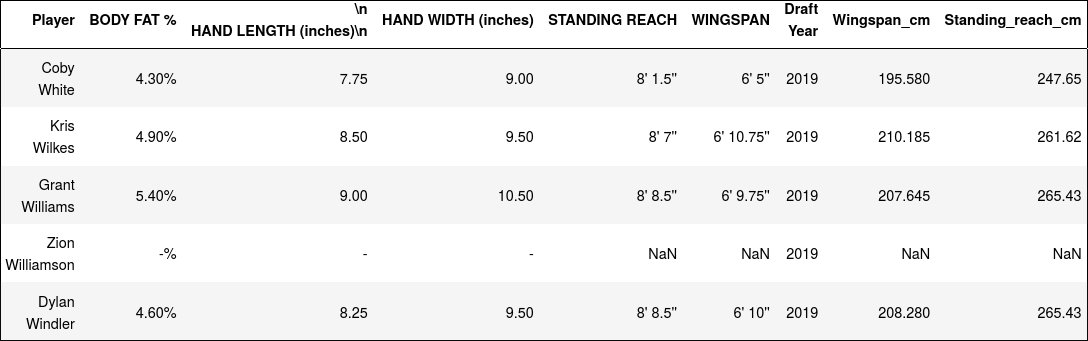
\includegraphics[scale=0.32]{nba_at.jpg}
\centering
\end{figure}

There are 1350 entries in the Draft Combine Anthro datasets. However, not all players in this dataset are NBA players. Therefore, I perform a left join between the NBA regular season dataset with this dataset to complete the physique dataset.

In the similar manner, I retrieve the PER data. After scraping html data for multiple times, I became relatively efficient at this skill.

\section{Data Checking}

There are entries in my dataset that are problematic. They are Guy Rucker and Xavier Silas, whose draft number is leave empty in the original dataset. After looking for their information online, I change their draft number to Undrafted.

\section{Data Exploration}
In this section, I use Rstudio to draw plots and explore data.
\subsection{The distribution of Height and Weight}
The distribution of \textbf{Height} for all players from 2000 to 2020 is shown in Figure 4. This distribution is skewed to the right, and the most popular height range is from about 195 to 210 centimeters. The tallest players are Yao Ming and Shawn Bradley (7f6 or 2.29m), while the shortest player is Earl Boykins (5f5 or 1.65m)

\begin{figure}[h]
\caption{Density plot of Height}
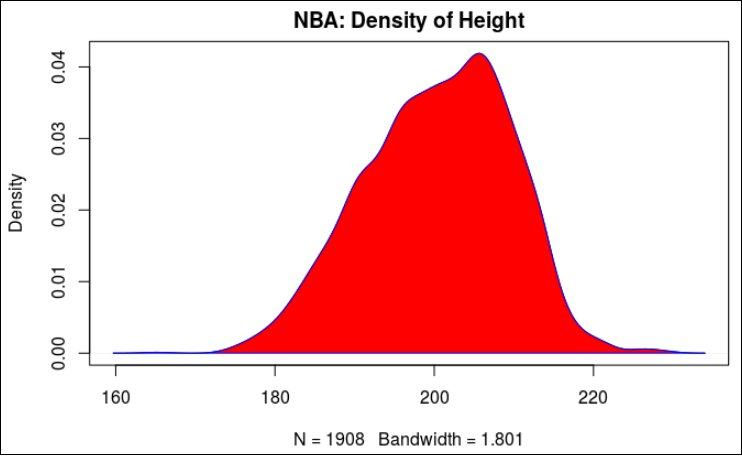
\includegraphics[scale=0.3]{dsoh.jpg}
\centering
\end{figure}

\begin{figure}[h]
\caption{Density plot of Height before vs after 2005}
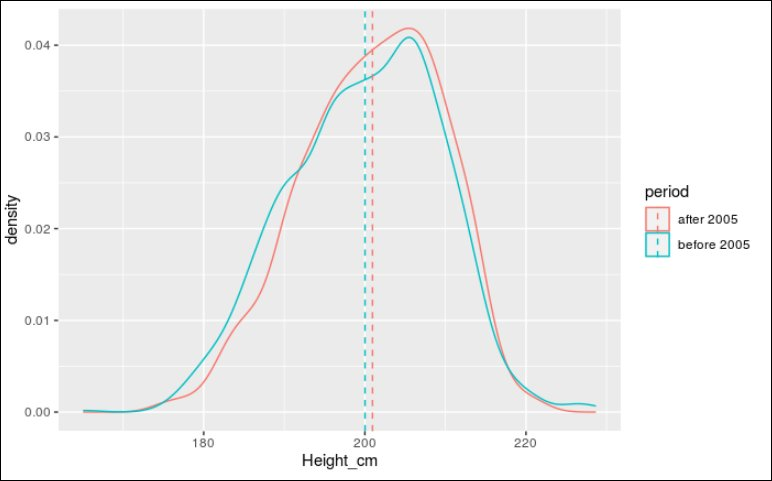
\includegraphics[scale=0.33]{hebf05.jpg}
\centering
\end{figure}

As the basketball game progresses, I expect to see the younger generation dominate the older in height. I used the draft year 2005 to split players into 2 groups to compare their height distribution. The result, shown in Figure 5, seems to confirm my speculation. The height mean of the younger group (200.9cm) is slightly higher than that of the older (200.2cm). The most height distribution of the young is also more tightened to the middle and shifted to the right, compared to the line for the older group, which implies that players drafted after 2005 are generally taller than their older counterpart.

\begin{figure}[h]
\caption{Distribution of Weight}
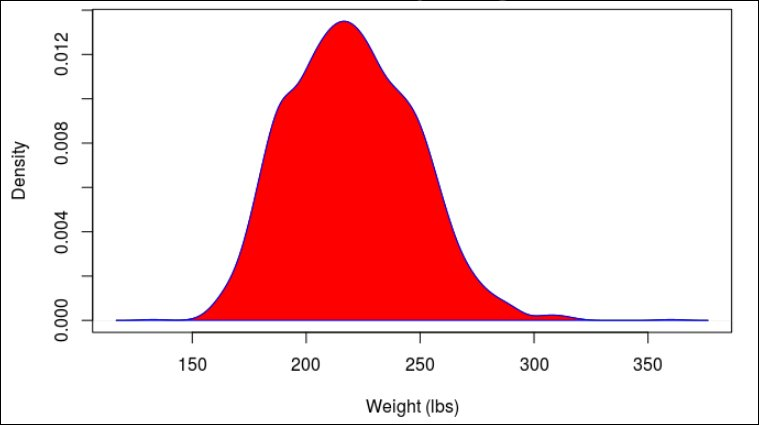
\includegraphics[scale=0.33]{dsow.jpg}
\centering
\end{figure}

\begin{figure}[h]
\caption{Density plot of Weight before vs after 2005}
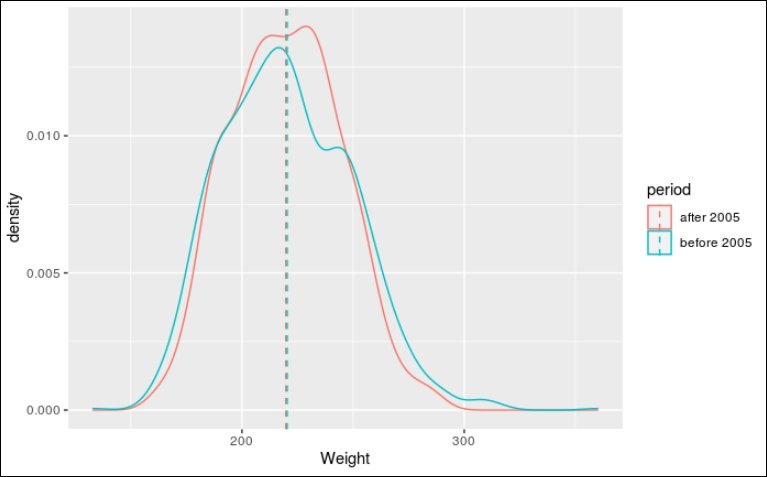
\includegraphics[scale=0.33]{webf05.jpg}
\centering
\end{figure}
I address the same question for \textbf{Weight}, and the result is shown in Figure 6 and Figure 7. The most popular weight range is about 200-230 pounds, and the mean weight for two group are roughly similar. However, the distribution of weight for the younger group are more tightened to the middle, implying a higher percentage of the heavier players, compared to the players drafted before 2005.




To conclude this section, I plotted to see how \textbf{Height} and \textbf{weight} are correlated, using a scatter plot.
\begin{figure}[h]
\caption{Height and Weight}
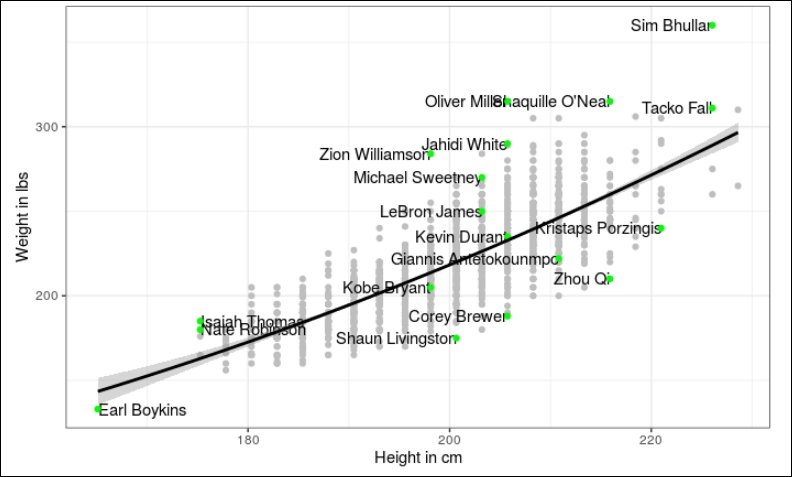
\includegraphics[scale=0.33]{hvw.jpg}
\centering
\end{figure}

An apparent upward trend is seen in the relationship between \textbf{Height} and \textbf{Weight}. This chart also exposes the outliers in my dataset. There are players who are very heavy for their frame, namely Zion Williamson, Oliver Miller, Shaquille O'Neal, and Sim Bhullar. This can pose huge stress on their knees and ankles, leading to injuries. There are also players who are too skinny, such as Corey Brewer, Shaun Livingston, Zhou Qui and Kristaps Porzingis.

There is not enough wingspan data for all of the player in my dataset (the earliest draft combine data available is from 2000). Therefore I conclude this section and move to the next part.

\subsection{Draft Number and Height, Weight}

I attempt to find a relationship between \textbf{Draft Number} and \textbf{Height}. but there are no significant pattern found (see figure 9). The same can be said for the relationship between Weight and Height
\begin{figure}[h]
\caption{Draft Number vs Height, Weight}
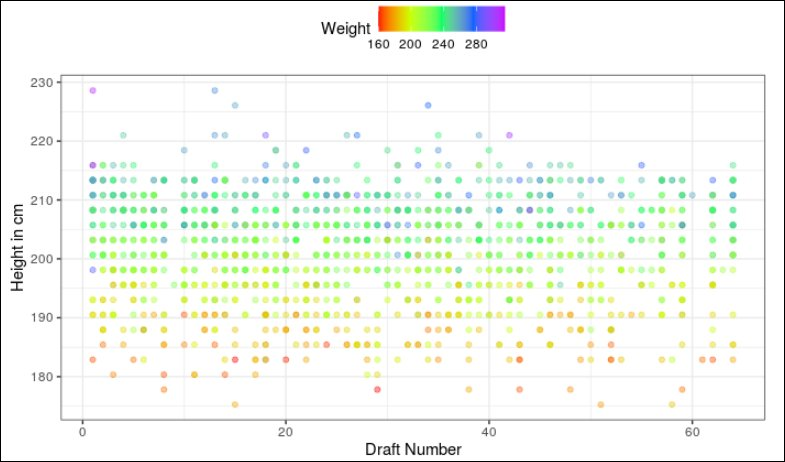
\includegraphics[scale=0.34]{hvdrf.jpg}
\centering
\end{figure}

\subsection{Nationality and Physique}
In 1908 entries in my dataset, there are only 377 foreign players (players who are not from the US). My theory is that foreign players must be physically dominant in order to be noticed by the NBA scouts. 

\begin{figure}[h]
\caption{Height of US vs non-US players}
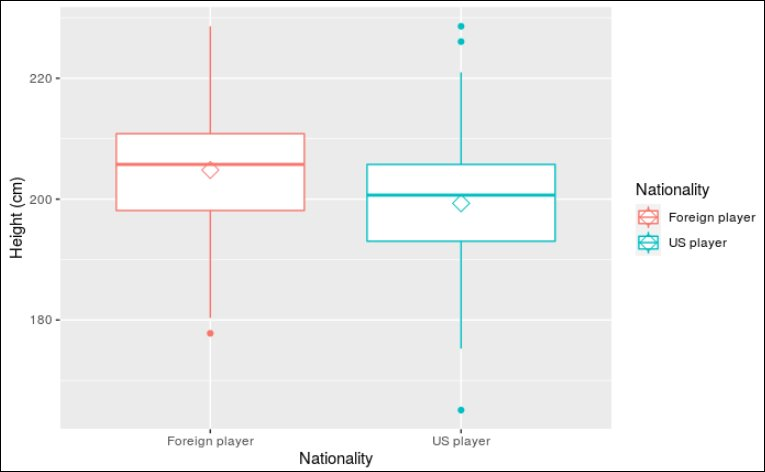
\includegraphics[scale=0.33]{fush.jpg}
\centering
\end{figure}

\begin{figure}[h]
\caption{Weight of US vs non-US players}
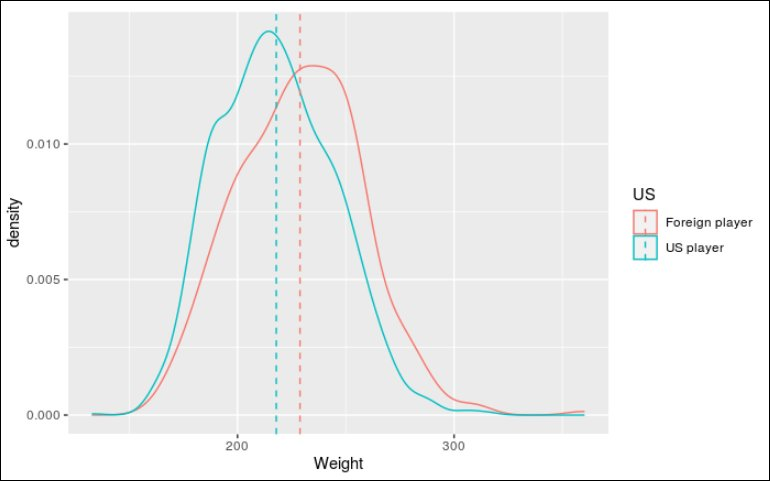
\includegraphics[scale=0.33]{fusw.jpg}
\centering
\end{figure}

It is convincing from the density distribution plots that non-US players are more dominant in height and weight: their distribution are shifted to the right of the US counterpart, and comparisons for mean height and weight also agree with my speculation.

\subsection{Physique and PER}
In this section, I will use the PER data for the
 regular season 2018-2019 and 2005-2006 for comparison. I hope to see some differences between two seasons as the game is supposedly modernized now.
\bibliographystyle{apacite}
\bibliography{nbabib}


\end{document}
